% ==========================================
% SECTION 5: INTERIOR AND CLOSURE (CONTINUED)
% ==========================================

\begin{spoken-clean}[00:00:00 - 00:01:32]
\inlinemetanote{The lecturer is writing the definitions of interior, closure, and boundary on the right chalkboard}
\end{spoken-clean}

\begin{math-stroke}[Definition: Interior, Closure, and Boundary]
\setcounter{theorem}{44}
\begin{definition}[Interior, Closure, and Boundary]\label{def:interior-closure-boundary}
Given a set $\Omega \subseteq X$ in a metric space $(X, d)$:
\begin{itemize}
    \setcounter{enumi}{0} \item The \emph{interior} of $\Omega$, denoted $\operatorname{int}(\Omega)$ or $\Omega^\circ$, is the largest open set contained in $\Omega$. Formally, it is the union of all open subsets of $\Omega$:
    \[ \operatorname{int}(\Omega) = \Omega^\circ = \bigcup \{ U \subseteq \Omega \mid U \text{ is open} \} \]
    \item The \emph{closure} of $\Omega$, denoted $\overline{\Omega}$, is the smallest closed set containing $\Omega$. Formally, it is the intersection of all closed sets containing $\Omega$:
    \[ \overline{\Omega} = \bigcap \{ A \supseteq \Omega \mid A \text{ is closed} \} \]
    Equivalently, it is the set of all points that can be reached as limits of sequences in $\Omega$:
    \[ \overline{\Omega} = \{ x \in X \mid \exists (x_n)_{n \ge 0} \subseteq \Omega \text{ s.t. } x_n \to x \} \]
    \item The \emph{boundary} of $\Omega$, denoted $\partial \Omega$, is the set difference between the closure and the interior:
    \[ \partial \Omega = \overline{\Omega} \setminus \Omega^\circ \]
\end{itemize}
\end{definition}
\end{math-stroke}

\begin{spoken-clean}[00:01:32 - 00:02:29]
Given a set $\Omega \subset X$, $(X, d)$ is a metric space. I define the interior of $\Omega$. This is called the interior of $\Omega$. This is by definition the largest open set contained in $\Omega$. So, you have your set $\Omega$ and you look at all the open sets that are contained and you get the largest one is the union of all the open sets that contain $\Omega$ (i.e., actually that are contained in $\Omega$). This is the interior.
\end{spoken-clean}

\begin{spoken-clean}[00:02:29 - 00:03:43]
Now, I also define the closure, that you know from $\mathbb{R}$, the closure of some set is the set of points $x$ in $X$ such that there exists some sequence $x_n$ such that the whole sequence is contained in $\Omega$ and then the sequence converges to $x$. You can also define this as the intersection of all the closed sets that are bigger than $\Omega$ (i.e., that contain $\Omega$). So, the closure is the smallest closed set that contains $\Omega$.
\end{spoken-clean}

\begin{spoken-clean}[00:03:43 - 00:05:33]
And then their difference, this minus this, this is called the boundary and is denoted with this symbol, the del symbol. This is called the boundary of $\Omega$. And this boundary of $\Omega$ is the \qt{skin}. Right? And if you do any example in the plane, you will see what this is doing. So, the closure is taking all this set with the skin, including the inside. And then you are removing the inside. So, when you draw the --- for this set over here... \inlinemetanote{Points at the square example he is about to draw}
\end{spoken-clean}

\begin{math-stroke}[Example: The Square \texorpdfstring{$[0, 1) \times [0, 1)$}{[0, 1) x [0, 1)}]
Consider the set $\Omega = [0, 1) \times [0, 1) \subset \mathbb{R}^2$.
\begin{center}
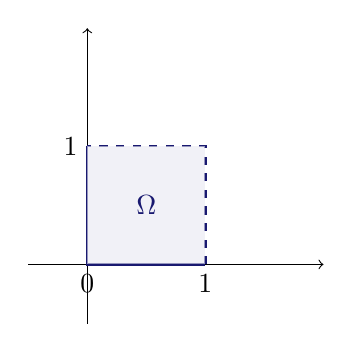
\begin{tikzpicture}[scale=1.5]
% \begin{ai-tikz-planner-invisible-content}
% 1. Background: Axes.
% 2. Midground: The square with mixed boundaries.
% 3. Foreground: Labels.
% \end{ai-tikz-planner-invisible-content}
    \draw[->] (-0.5,0) -- (2,0);
    \draw[->] (0,-0.5) -- (0,2);
    
    % The Set Omega
    \draw[thick, MidnightBlue] (0,1) -- (0,0) -- (1,0); % Solid boundaries
    \draw[dashed, thick, MidnightBlue] (1,0) -- (1,1) -- (0,1); % Dashed boundaries
    \fill[MidnightBlue!10, opacity=0.6] (0,0) rectangle (1,1);
    
    \node[MidnightBlue] at (0.5, 0.5) {$\Omega$};
    \node[below] at (0,0) {$0$};
    \node[below] at (1,0) {$1$};
    \node[left] at (0,1) {$1$};
\end{tikzpicture}
\end{center}

\begin{explanation-of-steps}
The set $\Omega$ includes its bottom and left edges (solid lines) but excludes its top and right edges (dashed lines).
\end{explanation-of-steps}
\end{math-stroke}

\begin{spoken-clean}[00:05:33 - 00:07:55]
So, how do you draw this example? It would be something like this, right? \inlinemetanote{Draws the square on the board} Is the inside of this square, but you are missing this part of the boundary and this part of the boundary. Now, can you see that these points satisfy this definition here? If I take a point here $x$ here, is on the boundary --- so is on the closure, sorry, is on the closure. Because I can take a sequence of points from the inside, from the red part (i.e., the shaded interior), that approaches $x$, right? But these points that are not in my set because I am excluding them, they are also on the closure. This point here $x$ over here is also on the closure. This belongs to the closure because I can take a sequence from here that approaches my point. Right?
\end{spoken-clean}

\begin{math-stroke}[Visualizing Interior, Closure, and Boundary]
For the set $\Omega = [0, 1) \times [0, 1)$:
\begin{center}
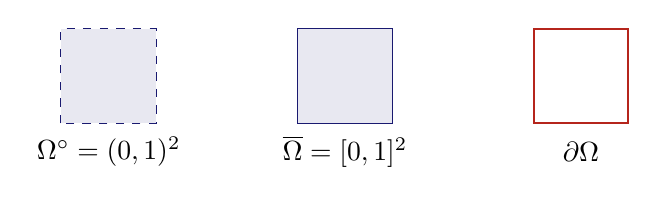
\begin{tikzpicture}[scale=1.2]
    % Interior
    \begin{scope}[shift={(0,0)}]
        \draw[dashed, thick, MidnightBlue] (0,0) rectangle (1,1);
        \fill[MidnightBlue!10] (0,0) rectangle (1,1);
        \node at (0.5, -0.3) {$\Omega^\circ = (0, 1)^2$};
    \end{scope}
    
    % Closure
    \begin{scope}[shift={(2.5,0)}]
        \draw[thick, MidnightBlue] (0,0) rectangle (1,1);
        \fill[MidnightBlue!10] (0,0) rectangle (1,1);
        \node at (0.5, -0.3) {$\overline{\Omega} = [0, 1]^2$};
    \end{scope}
    
    % Boundary
    \begin{scope}[shift={(5,0)}]
        \draw[thick, BrickRed] (0,0) rectangle (1,1);
        \node at (0.5, -0.3) {$\partial \Omega$};
    \end{scope}
\end{tikzpicture}
\end{center}
\begin{explanation-of-steps}
The interior $\Omega^\circ$ is the open square $(0, 1) \times (0, 1)$, which excludes all edges. The closure $\overline{\Omega}$ is the closed square $[0, 1] \times [0, 1]$, which includes all edges. The boundary $\partial \Omega$ is the set of all four edges of the square.
\end{explanation-of-steps}
\end{math-stroke}

\begin{spoken-clean}[00:07:55 - 00:08:52]
So, again all of these are perfectly common sense notions but that we can formalize and make perfectly rigorous just using these few axioms. And then, yes, I will prove maybe I will prove a lemma. \inlinemetanote{The lecturer erases the left chalkboard and prepares to write a new lemma}
\end{spoken-clean}

% \begin{ai-global-state-checkpoint-invisible-content}
% timestamp: 00:06:00
% topic: Definitions of Interior, Closure, and Boundary with the square example.
% board_state: def:interior-closure-boundary, ex:square-topology
% next_goal: State and prove the lemma characterizing open/closed sets via sequences.
% open_loops: none
% \end{ai-global-state-checkpoint-invisible-content}

% ==========================================
% SECTION 6: CHARACTERIZING OPEN AND CLOSED SETS VIA SEQUENCES
% ==========================================
\section{Characterizing Open and Closed Sets via Sequences}

\begin{spoken-clean}[00:08:52 - 00:10:12]
This lemma is called open and closed through sequences. How we determine if a set is open and closed using convergent sequences. So... \inlinemetanote{Starts writing the lemma on the board}
\end{spoken-clean}

\begin{math-stroke}[Lemma: Open and Closed Sets through Sequences]
\setcounter{theorem}{47}
\begin{lemma}[Open and Closed Sets through Sequences]\label{lem:open-closed-sequences}
Let $(X, d)$ be a metric space.
\begin{enumerate}
    \setcounter{enumi}{0} \item A subset $U \subseteq X$ is \emph{open} if and only if for every sequence $(x_n)_{n \ge 0}$ in $X$ that converges to a point $x \in U$, the sequence elements $x_n$ belong to $U$ \emph{eventually}.
    \[ U \text{ is open} \iff \left( \forall (x_n) \to x \in U \implies x_n \in U \text{ eventually} \right) \]
    \item A subset $A \subseteq X$ is \emph{closed} if and only if for every sequence $(x_n)_{n \ge 0}$ contained in $A$ that converges to a point $x \in X$, the limit $x$ also belongs to $A$.
    \[ A \text{ is closed} \iff \left( \forall (x_n)_{n \ge 0} \subseteq A \text{ s.t. } x_n \to x \implies x \in A \right) \]
\end{enumerate}
\end{lemma}
\end{math-stroke}

\begin{spoken-clean}[00:10:12 - 00:12:10]
So, this concept of \qt{up to finitely many exceptions} is very useful and is very, uh, nice to --- to say the thing shortly. And we give a name to this. And you have a more formal definition in the --- in the notes. So, when something happens --- when you have a sequence and some property, like for instance being in $U$, happens, is true up to finitely many exceptions, we say that this property happens \qt{eventually}.
\end{spoken-clean}

\begin{math-stroke}[Definition: Eventually]
\setcounter{theorem}{45}
\begin{definition}[Eventually]\label{def:eventually}
A property $P(x_n)$ is said to hold \emph{eventually} for a sequence $(x_n)_{n \ge 0}$ if it holds for all but finitely many terms. Formally:
\[ \exists N \in \mathbb{N} \text{ s.t. } \forall n \ge N, P(x_n) \text{ is true} \]
\end{definition}
\end{math-stroke}

\begin{proof}[Proof of Lemma \ref{lem:open-closed-sequences} (Part 1)]
\begin{spoken-clean}[00:12:10 - 00:15:50]
Proof of (1). So, I need to do two implications. First I will do this side ($\implies$) that is the one I draw here \inlinemetanote{points at the drawing of the open set $U$}. Assume that $U$ is open. And now take a point --- I'm just going to put in symbols the drawing that I did here. Take $x$ in $U$, any point. Then there --- by definition of open set, since $U$ is open, exists some $r$ positive such that the ball of radius $r$ centered at $x$ is contained in $U$. 

And now, since by assumption $x_n$ is converging to $x$, by definition of convergence, what was the definition of convergence? Remember: given any $\epsilon$ --- I called it in the definition --- this was the $\epsilon$ (i.e., the radius $r$), right? Given any $\epsilon$, now is $r$ but is the same. For $n$ large enough, bigger than a certain capital $N$, my sequence will belong to the ball of radius $\epsilon$ (i.e., $r$).
\end{spoken-clean}

\begin{math-stroke}[Forward Implication \texorpdfstring{$\implies$}{=>}]
Assume $U$ is open and $x_n \to x \in U$.
Since $U$ is open:
\[ \exists r > 0 \text{ s.t. } B(x, r) \subseteq U \]
Since $x_n \to x$, by the definition of convergence (using $\epsilon = r$):
\[ \exists N \in \mathbb{N} \text{ s.t. } \forall m \ge N, d(x_m, x) < r \]
This is equivalent to saying:
\[ \forall m \ge N, x_m \in B(x, r) \]
Since $B(x, r) \subseteq U$, it follows that:
\[ \forall m \ge N, x_m \in U \]
Thus, $x_n \in U$ eventually.
\end{math-stroke}

\begin{spoken-clean}[00:15:50 - 00:18:16]
Now I will prove the second implication ($\impliedby$). And I will prove this by contraposition. $A \implies B$ is equivalent to $\neg B \implies \neg A$, right? We know that. So, I will prove that \qt{not left} (i.e., $U$ is not open) implies \qt{not right} (i.e., there exists a sequence $x_n \to x \in U$ such that $x_n \notin U$ infinitely often).

So, now, let's do a bit of logic. What is the negation of $U$ open? Remember now, every time: what is the definition of $U$ open? $U$ open is: for every point in my set $U$, exists some radius such that the ball is contained in $U$. Now we do the negation. The negation of \qt{for every point} is \qt{exists a point}. So, $U$ is not open means exists $x$ in $U$ such that for every radius $r$ positive, the ball centered at $x$ with radius $r$ is not contained in $U$.
\end{spoken-clean}

\begin{math-stroke}[Backward Implication \texorpdfstring{$\impliedby$}{<=} (via Contraposition)]
We prove that if $U$ is not open, then there exists a sequence $x_n \to x \in U$ such that $x_n \notin U$ for all $n$.
        
\emph{Negation of Openness:}
\[ U \text{ is not open} \iff \exists x \in U \text{ s.t. } \forall r > 0, B(x, r) \not\subseteq U \]
The condition $B(x, r) \not\subseteq U$ means that the ball must contain at least one point from the complement $X \setminus U$:
\[ \forall r > 0, B(x, r) \cap (X \setminus U) \neq \emptyset \]
\end{math-stroke}

\begin{spoken-clean}[00:18:16 - 00:19:15]
\inlinemetanote{A student asks a question about notation} Ah, you mean this? \inlinemetanote{points at the $\subseteq$ symbol on the board} Is the same. You mean this? \inlinemetanote{points at the $\subset$ symbol} Is the same meaning. So, some people use the equality --- since it means the same, I save one line, right? But many --- this is very standard, many people just use this. So, I will use always this \qt{contained} without the equality sign.
\end{spoken-clean}

\begin{student-interaction}[Student Question]
You write the subset symbol without the extra line at the bottom. Does it have a meaning, like that it cannot be equal, or is that just notation?
\end{student-interaction}

\begin{spoken-clean}[continued]
It's just notation. In this course, $\subset$ and $\subseteq$ are used interchangeably to mean subset.
\end{spoken-clean}

\begin{spoken-clean}[00:19:15 - 00:21:15]
Okay, so back to the proof. Taking $r = 1/n$ for $n \ge 1$, I produced a sequence of points --- so these balls are smaller and smaller --- and these points $x_n$ (i.e., the $x_r$ for $r = 1/n$) are in balls closer and closer to $x$. So, they are converging to the point $x$. Right? So, I found a sequence that is converging to the point $x$ and that comes from the outside. But then, this is false (i.e., it contradicts the \qt{right} side of our implication). Because I'm saying that up to finitely many exceptions, the sequence should be contained in $U$. And all of the elements of this sequence are outside of $U$. So, this is false. This contradicts that $x_n$ belongs to $U$ eventually. And it ends the proof of this implication.
\end{spoken-clean}

\begin{math-stroke}[Constructing the Counter-Sequence]
For each $n \in \{1, 2, 3, \dots\}$, choose a radius $r_n = \frac{1}{n}$. By our assumption, there exists a point:
\[ x_n \in B(x, 1/n) \cap (X \setminus U) \]
This construction yields a sequence $(x_n)_{n \ge 1}$ such that:
\begin{enumerate}
    \setcounter{enumi}{0} \item $x_n \notin U$ for all $n$.
    \item $d(x_n, x) < \frac{1}{n} \to 0$, so $x_n \to x$.
\end{enumerate}
Since $x \in U$, the \qt{right} side of our lemma would require $x_n \in U$ eventually. However, our sequence is entirely outside $U$, which is a contradiction. Thus, $U$ must be open.
\end{math-stroke}
\end{proof}

\begin{spoken-clean}[00:21:15 - 00:24:04]
So, this proof by contraposition is very useful. Now, part (2) of the lemma is very similar. I leave it as an exercise. Try to do it, again. If you understood well the definitions and you can draw a picture of what's going on, this shouldn't be too difficult. But it can be a bit difficult at the beginning because there are a lot of new definitions. The best is to practice with these exercises. 

Let me put another exercise before continuity. Prove that if $(X, d)$ is a complete metric space and $A$ is a closed subset, then $A$ with the same distance restricted is complete. Example: we know that $\mathbb{R}^n$ is a complete metric space. Then any closed subset of $\mathbb{R}^n$ will be a complete metric space when you restrict the distance. And now you have all the ingredients to prove that. It's not too difficult. It's a good exercise.
\end{spoken-clean}

\begin{math-stroke}[Exercise: Completeness of Closed Subsets]
\begin{nice-box}[Exercise]
Prove the following proposition:
\begin{proposition}\label{prop:closed-subset-complete}
Let $(X, d)$ be a complete metric space. If $A \subseteq X$ is a closed subset, then the metric subspace $(A, d|_A)$ is also a complete metric space.
\end{proposition}
\end{nice-box}
\end{math-stroke}

\begin{spoken-clean}[00:24:04 - 00:25:30]
Okay, so I see the usual problem: when I see people that are very serious, I don't know if they are completely lost, if they find it super boring, or what is the problem. So, if someone has questions and wants to participate, we can slow down and ask questions. Otherwise, we continue with other stuff. We still need to do continuity, right? Well, let's make the pause. \inlinemetanote{The lecturer prepares for the break}
\end{spoken-clean}

\begin{lecture-break}[15-Minute Break]
The lecturer announces a break. The video resumes with the lecturer addressing the class after the break.
\end{lecture-break}

\begin{spoken-clean}[00:25:30 - 00:26:39]
Okay, I will start if you don't listen... well. So, may you forgive me for the stereotype, but when I studied mathematics in Barcelona, which is a Mediterranean country, people started on time the lecture. So, they were silent. We are in Switzerland, you should be like the champions of starting on time. And I'm seeing the contrary. I'm very surprised. Okay. And you know this is recorded, so this will be the proof of the misbehavior will be there for the history.
\end{spoken-clean}

% [SYSTEM] Video complete.